\documentclass[a4paper,UTF8]{article}
\usepackage{ctex}
\usepackage[margin=1.25in]{geometry}
\usepackage{color}
\usepackage{graphicx}
\usepackage{amssymb}
\usepackage{amsmath}
\usepackage{amsthm}
%\usepackage[thmmarks, amsmath, thref]{ntheorem}
\theoremstyle{definition}
\newtheorem*{solution}{Solution}
\newtheorem*{prove}{Proof}
\usepackage{multirow}
\usepackage{url}
\usepackage{enumerate}
\usepackage{algorithm}
\usepackage{algorithmic}
\renewcommand{\algorithmicrequire}{\textbf{Input:}}
\renewcommand{\algorithmicensure}{\textbf{Procedure:}}
\renewcommand\refname{参考文献}
\usepackage{caption,subcaption}
\usepackage{cite}
%--

%--
\begin{document}
\title{实验2. 隐马尔科夫模型实践}
\author{MF1733034,李青坪,\url{lqp19940918@163.com}}
\maketitle

\section*{综述}
	本次试验将实现隐马尔科夫模型\cite{周志华2016机器学习}( Hidden Markov Model, HMM),并将其应⽤在⾦融时序数据分析与预测⽅⾯。具体⽽⾔,对于⼀个已经训练好的 HMM,实现⼀个维特⽐算法,通过动态规划的思想对模型进⾏推断,其次,如果 HMM 的参数未知,则需要通过数据进⾏学习与训练,这⾥将部分实现 Baum–Welch\_algorithm.你将负责其中两个关键函数: HMM 的前向与后向算法。最后,利⽤⾃⼰从零开始写好的 HMM,进⾏股票的涨跌预测(for fun), 我们将预测中国某⽀与 AI 相关的股票的⾛势。
	
	对于单只股票数据,我们每⽇可以观测到的值可以是涨、跌,不涨不跌(相对于昨天的
收盘价)三种情况。这⾥将观测的涨跌平编码为 0,1,2 三种取值( 0:跌, 1:涨, 2:平)。
我们假设股票的涨跌由内在的隐变量驱动(这是⼀个⼗分简化的假设),即⽜市或熊市。
换⾔之,⽜市(编码为 1)⽐较有可能驱动股票价格上涨,熊市(编码为 0)⽐较有可能驱
动股票下跌。换⾔之,在本 HMM 模型中,隐变量仅仅是 1 维的 0/1 离散状态。
	
\section*{实验一.}
	\subsection*{维特比算法的概念}
		维特比算法是一种动态规划算法,它用于寻找最有可能产生观测事件序列的维特比路径——隐含状态序列,特别是在马尔可夫信息源上下文和隐马尔可夫模型中。维特比算法是针对一个特殊的图——篱笆网络的有向图而提出的,可以从图中找到最短路径,包括数字通信、语音识别、机器翻译等用到隐马尔可夫模型的技术都可以用维特比算法来解码。
	\subsection*{维特比算法的实现}
		给定隐马尔可夫模型的参数$ \lambda =[\textbf{A},\textbf{B},\pmb{\pi}] $,$ \textbf{A} $表示状态转移概率矩阵,$ a_{ij} $表示状态i转换到状态j的概率;$ \textbf{B} $表示输出观测概率矩阵,$ b_{ij} $表示根据状态i获得观测值$ o_j $的概率;$ \pmb{\pi} $表示初始状态概率,X表示观测序列\{$ x_1 $,$ x_2 $,...,$ x_T $\},S表示具有N个状态的状态空间。
		
		最有可能产生的状态序列Y=\{$ y_1 $,$ y_2 $,...,$ y_T $\}由以下递推关系给出:
		\begin{align*}
			&V_{1,k} = p(x_1|k)*\pi_k \\
			&V_{t,k} = p(x_t|k)*max_{y\in S}(a_{y,k}*V_{t-1,y})
		\end{align*}
		设path记录从每一个状态开始,最有可能到达的路径。对于某一状态y找到使$ V_{t,y} $最大的上一个状态state,则将[y]加入path[state]中,直到走完一整条观测序列,找到T时刻最大概率所对应的状态s,则path[s]即为最有可能的状态路径。

\section*{实验二.}
	\subsection*{Forward算法的实现}
		使$ \alpha_i(t) = p(X_1=x_1,X_2=x_2,...,X_t=x_t,Y_t=i|\lambda)$表示在t时刻,处于状态i,且观测到\{$ x_1,x_2,...,x_t $\}序列的概率。$ \alpha_i(t) $的值由以下式子递归得出:
		\begin{align*}
			&\alpha_i(1) = \pi_i b_i(x_1) \\
			&\alpha_i(t+1) = b_i(x_{t+1}) \sum_{j=1}^N \alpha_j(t)a_{ji}.
		\end{align*}
		Forward算法与维特比算法区别在于:前者是求出在t-1时刻,状态空间里面所有的状态能够在t时刻转移到状态i的概率之和作为$ \alpha_i(t) $;后者是求出在t-1时刻,状态空间中的某一状态y,y能够在t时刻转移到状态i的概率最大,$ V_{t,y} $则为该最大概率。前者用于训练HMM模型,后者是用于利用训练后的HMM模型根据观测序列计算最有可能出现的状态序列。

\section*{实验三. }
	使$ \beta_i(t) = p(X_{t+1}=x_{t+1},X_{t+2}=x_{t+2},...,X_T=x_T|Y_t=i,\lambda)$在时刻t,给定开始状态i,观测到结尾部分序列的\{$x_{t+1},x_{t+2},...,x_T$\}的概率。可通过以下式子计算$ \beta_i(t) $:
	\begin{align*}
		&\beta_i(T) = 1 \\
		&\beta_i(t) = \sum_{j=1}^N \beta_j(t+1) a_{ij} b_j(x_{t+1}).
	\end{align*}
	$ \beta_i(t) $表示的意思就是,在t+1时刻,状态空间中的所有状态能够在t时刻从状态i转移过来的概率之和。
\section*{实验结果}
	实验中,通过Baum–Welch算法训练出HMM模型,并利用维特比算法进行推断,预测股价的涨跌。执行HMM\_test.py脚本,验证代号为002415的股票在今年的预测准确度,实验结果表明,准确度在64.7\%左右。如图1所示:
	
\begin{figure}[htbp]
\centering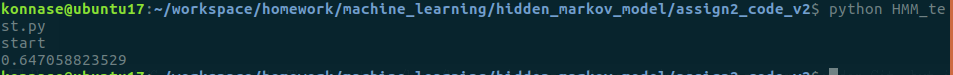
\includegraphics[width=5in]{result.png}
\caption{实验结果}
\label{fig:1}
\end{figure}
	
\renewcommand\refname{参考文献}
\bibliographystyle{plain}
\bibliography{assign2_report}
\end{document}